\documentclass{beamer}
    \usefonttheme{serif}
\usepackage{fontspec}
    \setmainfont{MLMRoman10}
    \setsansfont{MLMSans10}
    \setmonofont{MLMMono10}
\usepackage{verbatim}

\title{Is Detokenization All In The Head?}
\subtitle{An Interventional Study of Specialized Attention Heads \\ in Early Word Reconstruction}
\author{Gustaf Gren}
\date{Results}

\begin{document}

\begin{frame}
  \titlepage
\end{frame}

\begin{frame}{Detokenization in LLMs}

Tokenization can split up words non-coherently;\\
e.g.\ \texttt{['H',~'eming',~'way']}

\bigskip
\begin{itemize}
\item[\textbf{RQ1}] Do a few attention heads (5\%) drive whole-word representations in LLMs?
\item[\textbf{RQ2}] How does tokenizer choice affect these representations and robustness to ablation?
\item[\textbf{RQ3}] How does model size affect these representations and robustness to ablation?
\end{itemize}

\end{frame}

\begin{frame}{How to test that?}

\begin{block}{\textbf{Identification}}
    Identify candidate attention heads (prev. update)
\end{block}

\bigskip
\begin{block}{\textbf{Ablation}}
    \begin{itemize}
        \item Zero out $n$ attention heads in chosen layers.
        \item $n$ random head ablation in the same layers.
        \item Compare targeted vs.\ random ablation vs.\ clean run.
    \end{itemize}
\end{block}

\end{frame}

\begin{frame}{The Task}
\begin{exampleblock}{Example token sequence}
\small{
\texttt{['Sal', ' Paradiso', ' lives', ' in', ' Pat', \textcolor{red}{'erson'}]}
}
\end{exampleblock}

\bigskip
\begin{block}{Activation Patching}
Take the hidden state from each layer and insert it as $X$ into a fixed prompt to reconstruct the original full word.
\end{block}

\medskip
\texttt{"Repeat the following word: \textcolor{red}{X}, \textcolor{red}{X}, \textcolor{red}{X},"} \\
\end{frame}

\begin{frame}{RQ1: Targeted vs.\ Random Ablation}
\begin{itemize}
    \item Targeted ablation suffers large performance drop compared to baseline.
    \item Random ablation has minor effect in general.
\end{itemize}

\bigskip
\textbf{For example}: in \texttt{qwen2.5}/English we drop from 0.81\ in the clean
condition to 0.01 after targeted ablation, but we only drop to 0.80 after
random ablation.

\end{frame}

\begin{frame}{RQ2: Tokenizer \& Language}
\begin{center}

\includegraphics[width=0.55\linewidth]{plots/toksuite_stack/layerwise_retrieval_pooled_mean.pdf}
\end{center}
\end{frame}

\begin{frame}{RQ2: Tokenizer \& Language --- English}
\begin{center}

\includegraphics[width=0.55\linewidth]{plots/toksuite_stack/layerwise_retrieval_lang_english.pdf}
\end{center}
\end{frame}

\begin{frame}{RQ3: Model Size}
\begin{center}
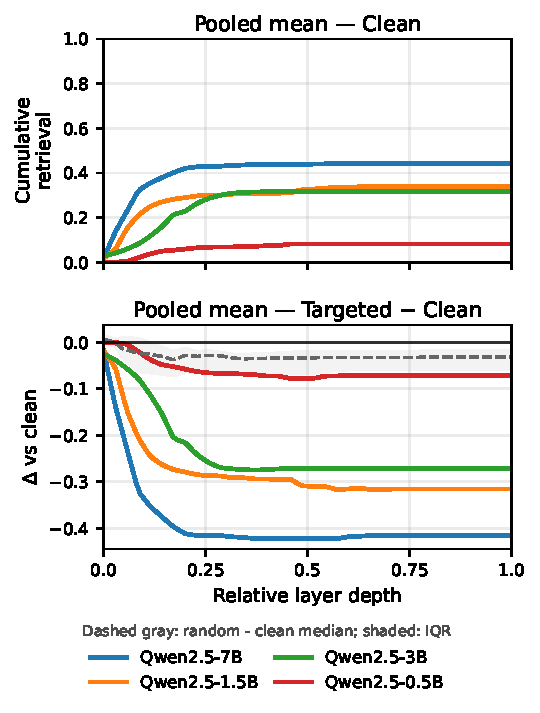
\includegraphics[width=0.55\linewidth]{plots/qwen_stack/layerwise_retrieval_pooled_mean.pdf}
\end{center}
\end{frame}

\begin{frame}{RQ3: Model Size}
\begin{center}
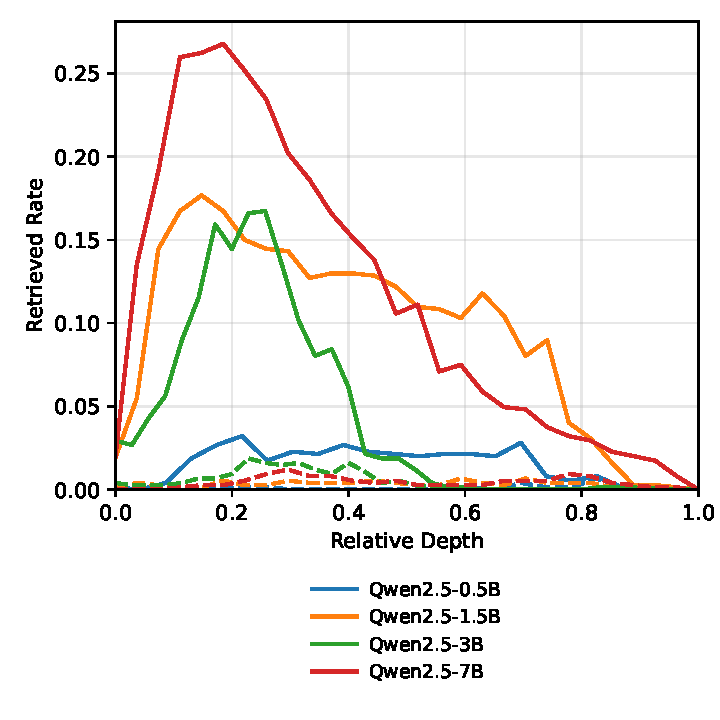
\includegraphics[width=0.7\linewidth]{plots/qwen_rr/retrieved_rate_model_comparison/pooled/retrieved_rate_model_comparison_pooled.pdf}
\end{center}
\end{frame}

\begin{frame}{Takeaways}
\begin{itemize}
\item Specific attention heads drive multi-token word representations.
\item Zeroing these heads \textbf{hurts retrieval} (random not so much)>
\item Larger models show \textbf{specialized attention} and better retrieval.
\item Tokenizer design impacts learning efficiency for representations.
\end{itemize}
\end{frame}

\end{document}
